\chapter{WAN concepts}

\section{WAN Technologies overview}

\subsection{Topology}

A WAN operates beyond the geographic scope of a LAN. WANs are used to interconnect the enterprise LAN to remote LANs in branch sites and telecommuter sites. A WAN is owned by a service provider whereas a LAN is typically owned by an organization. An organization must pay a fee to use the WAN service provider’s network services to connect remote sites.\\

\begin{figure}[hbtp]
\centering
\subfigure[Point-to-point]
	{
		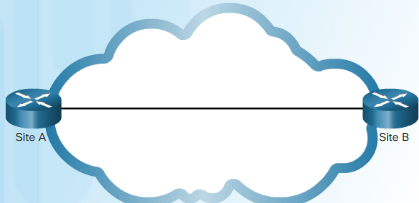
\includegraphics[width=0.4\textwidth]{pictures/WANtopology1.PNG}
		\label{WANtopology1}	
	}
\subfigure[Hub-and-Spoke]
	{
		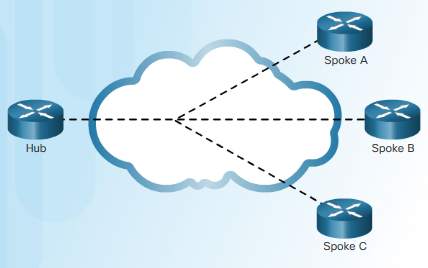
\includegraphics[width=0.4\textwidth]{pictures/WANtopology2.PNG}
		\label{WANtopology2}
	}
\subfigure[Full Mesh]
	{
		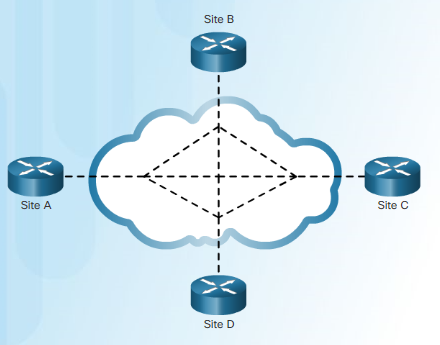
\includegraphics[width=0.4\textwidth]{pictures/WANtopology3.PNG}
		\label{WANtopology3}
	}
\subfigure[Dual-homed]
	{
		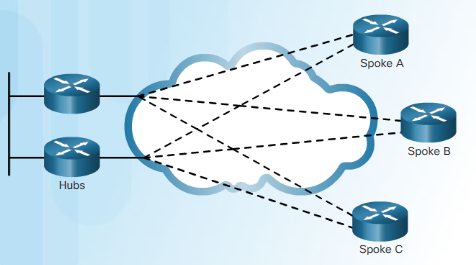
\includegraphics[width=0.4\textwidth]{pictures/WANtopology4.PNG}
		\label{WANtopology4}
	}
\caption{Four common WAN topologies}
\end{figure}

\paragraph{Point-to-Point topology} employs a point-to-point circuit between two endpoints (Figure \ref{WANtopology1}). Typically involves a dedicated leased-line connection such as a T1/E1 line.

\paragraph{Hub-and-Spoke} An example of a single-homed topology. Applicable when a private network connection between multiple sites is required. A single interface to the hub can be shared by all spoke circuits (Figure \ref{WANtopology2}).

\paragraph{Full Mesh} A disadvantage of the hub-and-spoke topology is that all communication has to go through the hub. With a full mesh topology using virtual circuits, any site can communicate directly with any other site (Figure \ref{WANtopology3}). A disadvantage is the large number of virtual circuits that need to be configured and maintained.

\paragraph{Dual-homed Topology} Provides redundancy and load balancing, however more expensive to implement than single-homed topologies(Figure \ref{WANtopology4}). Requires additional networking hardware including routers and switches. More difficult to implement since they require complex configurations.

\subsection{Terminology}

WAN operations focus primarily on the Layer 1 and 2 of the OSI Model. One primary difference between a WAN and a LAN is that a company must subscribe to an outside WAN service provider to use WAN carrier network services.\\

\begin{figure}[hbtp]
\caption{Common WAN terminology}\label{terminology}
\centering
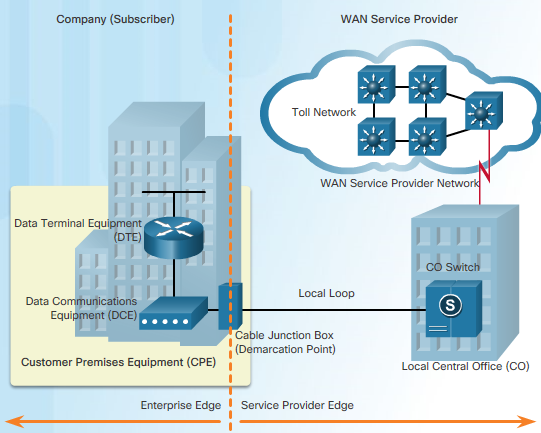
\includegraphics[ width=0.7\textwidth ]{pictures/DCE.PNG}
\end{figure}

Terminology commonly used to describe WAN connections (Figure \ref{terminology}):

\begin{itemize}
\item \textbf{Customer Premises Equipment (CPE)} Consists of devices and inside wiring located on the enterprise edge connecting to a carrier.

\item \textbf{Central Office (CO)} is the local service provider facility that connects the CPE to the provider network.

\item \textbf{Local Loop (last mile)} is the actual copper or fiber cable that connects the CPE to the CO.

\item \textbf{Data Terminal Equipment (DTE)} is usually a router that pass the data from a customer network to DCE.

\item \textbf{Data Communications Equipment (DCE)} is usually a modem that puts data on the local loop by converting digital signals into analog signals. It connects subscribers to the ISP provider.

\item \textbf{Demarcation Point} is a point established in a building to separate customer equipment from service provider equipment. It is the place where the responsibility for the connection changes from the user to the service provider.

\item \textbf{Toll network} consists of the longhaul, all-digital, fiber-optic communications lines and other equipment inside the WAN provider network.
\end{itemize}

\begin{figure}[hbtp]
\caption{WAN devices}\label{Device}
\centering
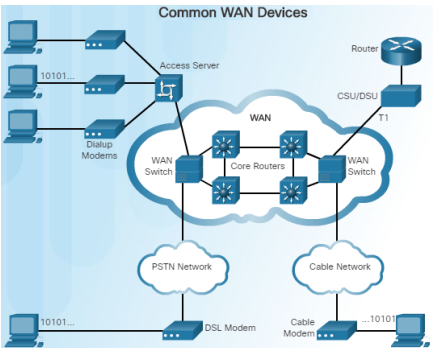
\includegraphics[scale=1]{pictures/Device.PNG}
\end{figure}

There are many types of devices that are specific to WAN environments (Figure \ref{Device}):

\begin{itemize}
\item \textbf{Dialup modem} converts (modulates) the digital signals (produced by a computer) into analog signals (voice frequencies).

\item \textbf{Broadband modem} converts the digital signals into analog signals transferred via high-speed DSL or cable Internet service.

\item \textbf{Access server} controls and coordinates dialup modem, dial-in and dial-out user communications.


\item \textbf{CSU/DSU} is only used for Leased lines. The CSU provides termination for the digital signal and ensures connection integrity through error correction and line monitoring. The DSU converts line frames into frames that the LAN can interpret and vice versa.
\end{itemize}

WAN technologies are either circuit-switched or packet-switched:

\paragraph{Circuit Switching} dynamically establishes a \emph{dedicated virtual connection} for voice or data between a sender and a receiver. Communication can't start until the connection is established through the service provider network. The two most common types of circuit-switched WAN technologies are \textbf{PSTN} and \textbf{ISDN}.

\paragraph{Packet Switching} splits traffic data into packets packet that are routed over a shared network. A circuit does not need to be established and many pairs of nodes can communicate over the same channel. Packet switching costs less than circuit switching, however, latency and jitter are greater in packet-switching networks. There are two approaches to packet-switched network link determination:

\begin{itemize}
\item \textbf{Connectionless systems:} Full addressing information must be carried in each packet. The \textbf{Internet} is an example of a connectionless system. 
\item \textbf{Connection-oriented systems:} The network predetermines the route for a packet, and each packet only has to carry an identifier. An example of a connection-oriented system is \textbf{Frame Relay} (DLCIs are the identifiers).
\end{itemize}

\section{WAN connection}

There are several WAN access connection options (figure \ref{WANaccess}) that ISPs can use to connect the local loop to the enterprise edge.\\

\begin{figure}[hbtp]
\caption{WAN access options}\label{WANaccess}
\centering
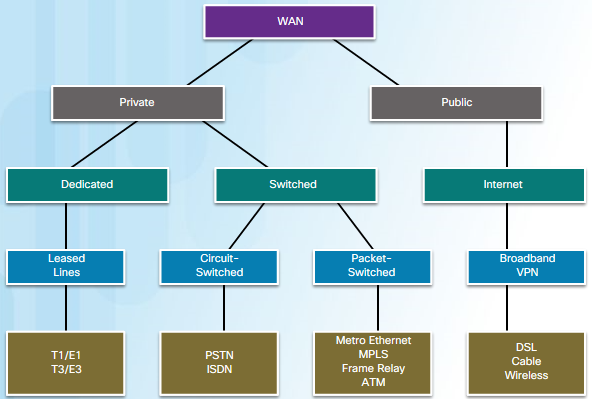
\includegraphics[ width=0.7\textwidth ]{pictures/WANaccess.PNG}
\end{figure}

Service provider networks are complex and consist mostly of high-bandwidth fiber-optic media, using SONET and SDH standard. A newer fiber-optic media development for long-range communications is called dense wavelength division multiplexing (DWDM).

\subsection{Private WAN Infrastructures}

\paragraph{Leased lines} are permanent dedicated point-to-point connections from the customer premises to the provider network. The term leased line refers to the fact that the organization pays a monthly lease fee to a service provider to use the line. Leased lines are simple to implement and offer high quality and availability but are generally the most expensive type of WAN access and has Limited flexibility.

\paragraph{Dialup}transport binary computer data through the voice telephone network using a modem. Dialup access is suitable when intermittent, low-volume data transfers are needed. The advantages of modem and analog lines are simplicity, availability, and low implementation cost. The disadvantages are the low data rates and a relatively long connection time. 

\paragraph{ISDN}is a \underline{circuit-switching} technology that enables the local loop of a PSTN (Public switched telephone network) to carry digital signals. It can provide additional capacity as needed on a leased line connection or can also be used as a backup. ISDN has declined in popularity due to DSL and other broadband services. There are two types of ISDN Interfaces: BRI (2 B-channels, 1 D-channel), PRI (23 B-channel, 1 D-channel)

\paragraph{Frame Relay}Frame Relay is a Layer 2 WAN technology used to interconnect enterprise LANs. A single router can be used to connect multiple sites using Private Virtual Circuits (PVCs) which can carry both voice and data traffic. Frame Relay creates PVCs which are uniquely identified by a data-link connection identifier (DLCI). The PVCs and DLCIs ensure bidirectional communication between one DTE device to another.

\paragraph{ATM} is built on a cell-based architecture rather than on a frame-based architecture. ATM cells are always a fixed length of 53 bytes, containing a 5-byte ATM header followed by 48 bytes of ATM payload. Small, fixed-length cells are well-suited for carrying voice and video traffic because this traffic is intolerant of delay. However, when the cell is carrying segmented network layer packets, the overhead is higher because the ATM switch must be able to reassemble the packets at the destination. 

\paragraph{Ethernet WAN}Originally Ethernet was not suitable as a WAN access technology because the maximum cable length was one kilometer. However, fiber-optic cables have made Ethernet a reasonable WAN access option. There are several benefits to an Ethernet WAN: Reduced expenses and administration, Easy integration with existing networks, Enhanced business productivity. Ethernet WANs have replaced Frame Relay and ATM.

\paragraph{MPLS} is a multiprotocol high-performance WAN technology that directs data from one router to the next. MPLS is based on short path labels rather than IP network addresses.  It uses labels which tell a router what to do with a packet. The labels identify paths between distant routers rather than endpoints, and while MPLS actually routes IPv4 and IPv6 packets, everything else is switched. Furthermore, MPLS can deliver any type of packet between sites and encapsulate them of various network protocols.

\paragraph{VSAT} is a solution that creates a private WAN using satellite communications in remote locations where there are no service providers that offer WAN service.

\subsection{Public WAN Infrastructures}

\paragraph{DSL}is an always-on connection technology that uses existing twisted-pair telephone lines to transport high-bandwidth data. A DSL modem converts an Ethernet signal from the user device to a DSL signal. Key components in the DSL connection: DSL modem (subscriber end) and DSLAM (ISP end). The advantage that DSL has over cable technology is that DSL is not a shared medium -- each user has a separate direct connection to the DSLAM.

\paragraph{Cable} Coaxial cable is widely used in urban areas to distribute television signals. Network access is available from many cable television providers. This allows for greater bandwidth than the conventional telephone local loop. Two types of equipment are required: CMTS (ISP end), and Cable Modem (subscriber end).

\paragraph{WiMAX} is a new technology that operates in a similar way to Wi-Fi, but at higher speeds, over greater distances, and for a greater number of users. It uses a network of WiMAX towers that are similar to cell phone towers. 

\paragraph{Satellite Internet}Typically used by rural users where cable and DSL are not available. Cable and DSL have higher download speeds, but satellite systems are about 10 times faster than an analog modem. 

\paragraph{VPN}is an encrypted connection between private networks over Internet. VPN uses virtual connections called VPN tunnels, which are routed through the Internet from the private network of the company to the remote site or employee host. There are several benefits to using VPN: cost savings, security, scalability, compatibility with broadband technology. There are two types of VPN access: 

\begin{itemize}
\item \textbf{Site-to-site VPN:} connect entire networks to each other, for example, connecting a branch
office network to a company headquarters network. 
\item \textbf{Remote-access VPN:} enable individual hosts, such as  extranet consumers, to access a company network securely over the Internet.
\end{itemize}

\paragraph{Dynamic Multipoint VPN (DMVPN)} is a Cisco software solution for building multiple VPNs. DMVPN is built on three protocols: NHRP, IPsec, and mGRE. NHRP is the distributed address mapping protocol for VPN tunnels. IPsec encrypts communications on VPN tunnels. The mGRE protocol allows the dynamic creation of multiple spoke tunnels from one permanent VPN hub.